% Une ligne commentaire débute par le caractère « % »

\documentclass[a4paper]{article}

% Options possibles : 10pt, 11pt, 12pt (taille de la fonte)
%                     oneside, twoside (recto simple, recto-verso)
%                     draft, final (stade de développement)

\usepackage[utf8]{inputenc}   % LaTeX, comprends les accents !
\usepackage[T1]{fontenc}      % Police contenant les caractères français
\usepackage[francais]{babel}  


\usepackage[a4paper,left=2cm,right=2cm]{geometry}% Format de la page, réduction des marges
\usepackage{graphicx}  % pour inclure des images

%\pagestyle{headings}        % Pour mettre des entêtes avec les titres
                              % des sections en haut de page

 \title{  Qui est-ce ?\\         % Les paramètres du titre : titre, auteur, date
  Projet de programmation}          
\author{Groupe \emph{Z}\\
  \emph{Frédéric,Laurent,Tony et Romain}\\
  \emph{git:git@gitlab.etu.umontpellier.fr:e20180001091/qui-est-ce.git}\\
  L2 informatique\\
  Faculté des Sciences\\
Université de Montpellier.}
\date{\today}             

\begin{document}

\maketitle                    % Faire un titre utilisant les données
                              % passées à \title, \author et \date

\begin{center}               % pour centrer 
  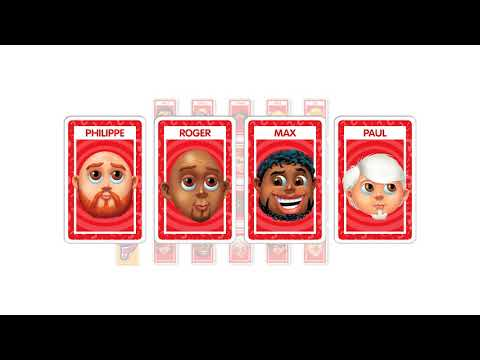
\includegraphics[scale=1]{img.jpg}   % insertion d'une image
\end{center}

\begin{abstract}     % Résumé du travail
Nous avons réalisé l'IHM et le jeu/générateur en parrallèle. De nombreux problèmes d'organisation et de git nous ont ralentis.
\end{abstract}

\section{Étape 1 : permettre à l'utilisateur de jouer}

\subsection*{Fonctionnalités de l'application : interactions possibles de l'utilisateur}

\paragraph*{}
Le jeu (de base)

Après avoir lancé le terminal, nous entrons notre nom, choissisons le plateau, puis mode facile ou difficile.

Une fois en jeu, nous pouvons coché des portrait (clic gauche) et accuser un personnage (clic droit)
En bas de la fenêtre, des bouttons nous permettent de créer notre question, de la poser puis voir la réponse.
Un haut, un petit menu vous permettra de sauvegarder la partie en cours, voir votre historique de question et abbandoner.

\paragraph*{}
Le générateur

Le joueur doit lancé le générateur par le terminal en choisisant en paramètre le thème.

En ce qui concerne les métadonnées (taille de la grille, des images), il est possible de les modifier si les valeurs par défaut ne conviennent pas.

Ensuite, l'utilisateur doit définir des attributs puis y ajouter des valeurs afin de les utiliser par la suite.

Par ailleurs, les attributs avec leurs valeurs peuvent être donner à des personnages.

Il n'y a pas d'autré pré-établi si ce n'est que il vous faut au moins un attribut avec au moins 1 valeur pour pouvoir la donner à un personnage. 

Nous avons la possibilité d'ajouter des attributs, d'ajouter des valeurs à ces attributs, modifier et supprimer. Ces Fonctionnalités ont des répercussions sur les personnage qui les portent.


\subsection*{Format du fichier JSON, contraintes éventuelles}
"metadonnees" Cette clé renvoie vers des données essentiels pour le bon fonctionnement de l'interface graphique.\\
"images" contient le chemin vers le dossier contenant les images depuis la racine du projet \\
"ligne" et "colonne" forment la taille de la grille\\
"largeurImage" et "hauteurImage" correspond à la définition de chaque portrait à l'écran (!= la définition réel des images dans le dossier)\\
"espacementPhoto" est l'espacement entre les portrait sur l'interface graphique\\
"possibilites"\\
Chaque clé correspond à la représentation d'un personnage.
Chaque personnage doit avoir les clés "fichier" et "nom".
Le reste des clés du personnages correspond aux noms de ces attributs.
Les clés des personnages sont associés à des liste pour permettre la multiplicité des valeurs.
Les personnages ont le même nombre d'attribut.

\begin{figure}
  \caption{Squelette type de nos fichier JSON}
  \centering
  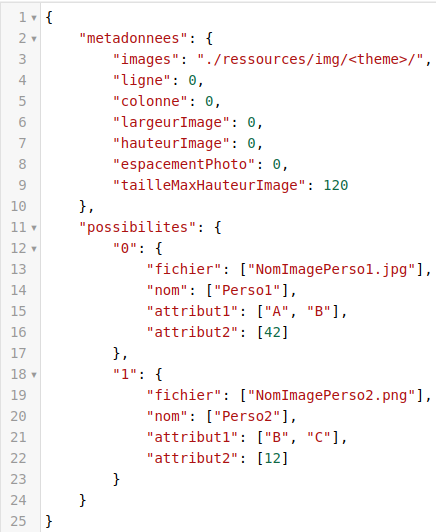
\includegraphics[scale=0.15]{./squeletteJSON.png}
\end{figure}

\clearpage
\subsection*{Description des structures de données, classes, variables}
\paragraph*{La classe Jeu} ne contient pas de logique. Elle sert simplement à réunir les autres objets dans un unique objet, facilité la création des objets et contient quelques méthodes "utiles".
La méthode calculeMapAttributsDomaine() renvoie les attributs et leurs valeurs sous forme de dictionnaire pour l'interface
Nous considérons que poser une question sur le nom d'un personnage et sur ses attributs sont philosophiquement différentes, par conséquent il d'un côté accuser() pour identifier ou pas notre personnage mystère et evaluer() pour poser des questions.

\begin{figure}
  \caption{Diagramme de classe du jeu}
  \centering
  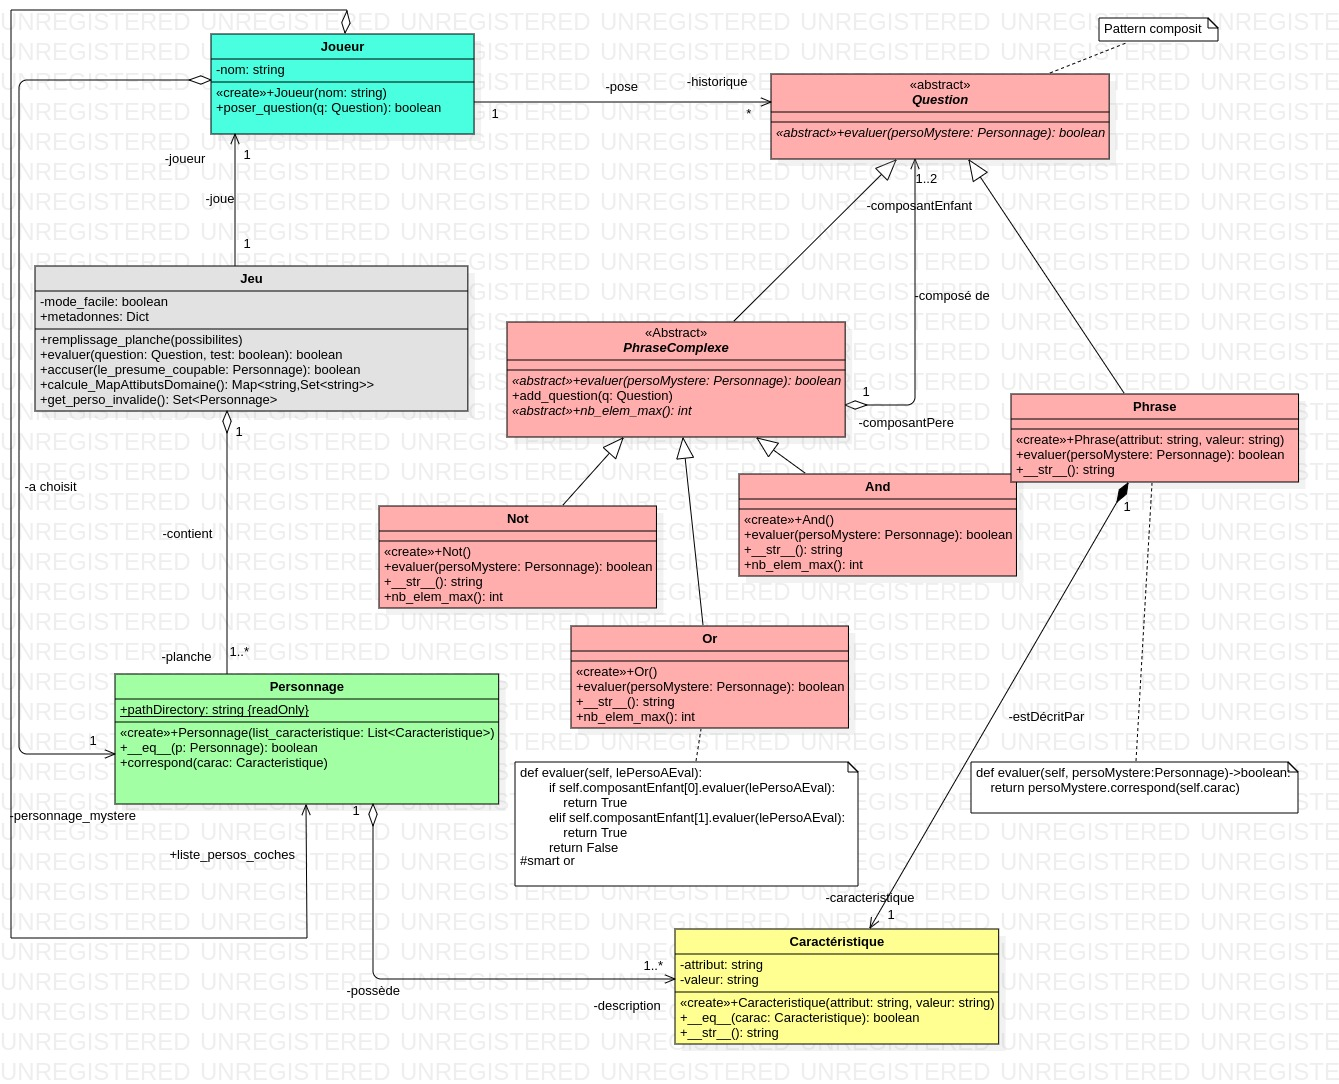
\includegraphics[scale=0.35]{./JeuClassDiagram.jpg}
\end{figure}

\clearpage
\subsection*{Description de la forme des requêtes traitées et un traitement.}
\begin{figure}
  \caption{Diagramme objet représentant une question}
  \centering
  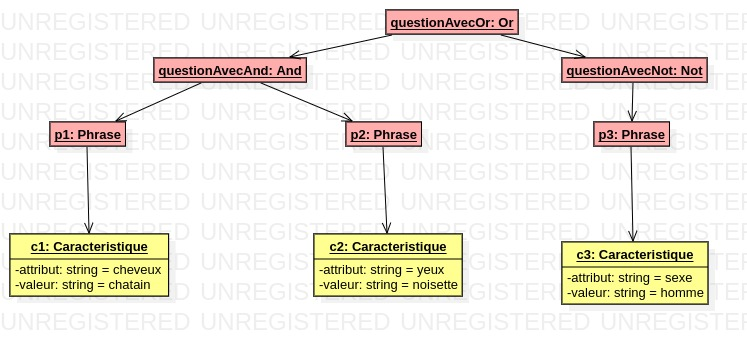
\includegraphics[scale=0.4]{./requetesObject.jpg}
\end{figure}
\paragraph*{}
Nous avons choisit d'utiliser un pattern composite pour représenter les questions.
En effet, la situation si prete bien. Puisque dans notre Qui-est ce?, nous voulons qu'un utilisateur puisse intéroger sur plusieurs choses à la fois tout en représetant sufisament précisement la complexité d'une question.
Nous voullons qu'une question puisse en contenir d'autre et être relié par un connecteur logique donné.
En cela, le composit pattern remplis notre besoin car une question est un arbre dont les différents nœuds sont des connecteurs logiques, et les vrais questions sont les feuilles de cette arbre. Et un sous arbre serait également une question valide.


\subsection*{Description du traitement effectué lors d'une requête.}
\begin{figure}
  \caption{Diagramme de séquence, le joueur pose une question}
  \centering
  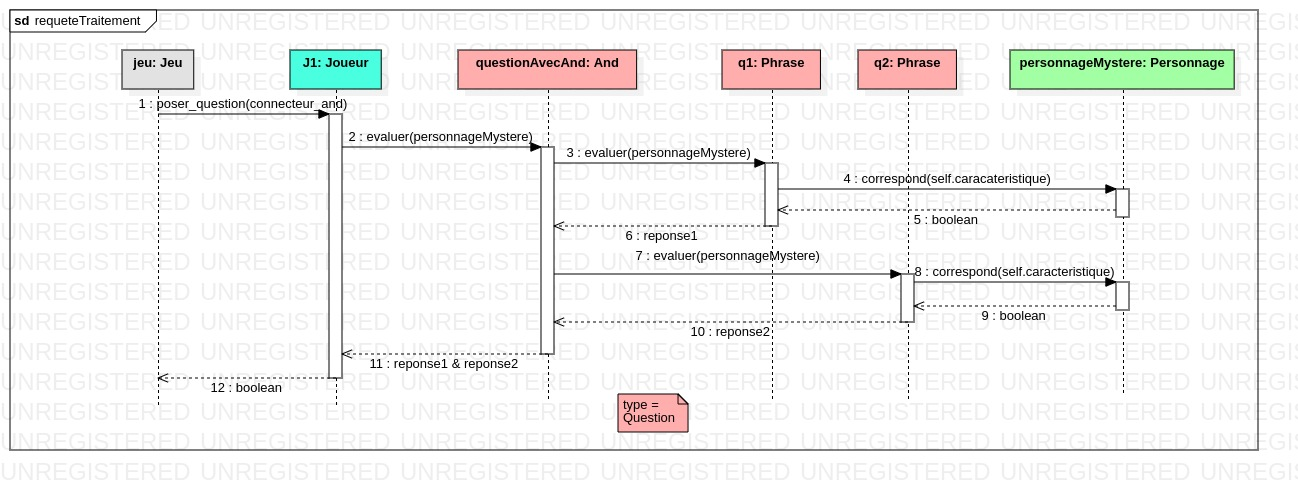
\includegraphics[scale=0.38]{./requeteTraitement.jpg}
\end{figure}

\paragraph*{}Lorsque que le joueur pose une question (1), l'objet J1 de type Joueur va passé le personnage mystère pour que la question qu'il veut posé puisse être évaluer.
La question questionAvecAnd va s'évaluer (2) récursivement avec ces enfants (3,7) jusqu'à qu'elle tombe sur une feuille. Les phrases au bout de l'arbre vérifie si ils correspond au personnage passé en argument (4,8).
\clearpage
\end{document}

